\section{Results}

\subsection{Miss-use modeling}

\begin{table}[h!]
\footnotesize
\centering
  \caption{Summary of cascades level population.}
\resizebox{\columnwidth}{!}{%
\begin{tabular*}{\textwidth}{c @{\extracolsep{\fill}} cccccccc}
\toprule

Model       &        &                & A/NR     & A/R      & B/NR     & B/R      & C/NR     & C/R       \\
%Recycling   &       &                & No       & Yes      & No       & Yes      & No       & Yes        \\
\midrule                                                                                                 
        &            & Feed $w\%$     & $0.71$   & $1.31$   & $0.71$   & $0.92$   & $0.71$   & $1.30$ \\
Level 0 & Assay      & Product $w\%$  & $3.97$   & $7.27$   & $3.97$   & $5.10$   & $3.97$   & $7.24$ \\
        &            & Tails $w\%$    & $0.28$   & $0.52$   & $0.28$   & $0.36$   & $0.28$   & $0.51$ \\
        & Cascades   & Impl. (Ideal)  & 25(26.5) & 25(26.5) & 24(26.4) & 25(26.3) & 25(26.5) & 25(26.2)  \\
\midrule                                                                                                 
        &            & Feed $w\%$     & $3.97$   & $11.48$  & $3.97$   & $6.29$   & $3.97$   & $11.64$ \\
Level 1 & Assay      & Product $w\%$  & $21.29$  & $53.30$  & $19.33$  & $27.98$  & $21.41$  & $55.12$ \\
        &            & Tails $w\%$    & $1.68$   & $5.93$   & $1.58$   & $2.54$   & $1.66$   & $5.88$ \\
        & Cascades   & Impl. (Ideal)  & 3(3.1)   & 4(3.1)   & 3(3.1)   & 3(3.1)   & 3(3.1)   & 4(3.4)    \\
\midrule                                                                                                 
        &            & Feed $w\%$     & $21.29$  & $53.3$   & $19.33$  & $31.09$  & $21.41$  & $55.12$ \\
Level 2 & Assay      & Product $w\%$  & $76.39$  & $94.70$  & $58.10$  & $72.31$  & $79.21$  & $96.37$ \\
        &            & Tails $w\%$    & $13.98$  & $47.81$  & $8.51$   & $14.91$  & $13.75$  & $49.65$ \\
        & Cascades   & Impl. (Ideal)  & 1(0.4)   & 1(0.4)   & 1(0.4)   & 1(0.5)   & 1(0.4)   & 1(0.4)   \\
\midrule                                                                                                 
        &            & Feed $w\%$     & $76.39$  & N.A.     & $58.10$  & $72.31$  & $79.21$  & N.A.      \\
Level 3 & Assay      & Product $w\%$  & $98.09$  & N.A.     & $88.92$  & $93.79$  & $98.86$  & N.A.      \\
        &            & Tails $w\%$    & $73.51$  & N.A.     & $35.01$  & $50.36$  & $76.60$  & N.A.      \\
        & Cascades   & Impl. (Ideal)  & 1(0.04)  & N.A.     & 1(0.09)  & 1(0.1)   & 1(0.04)  & N.A.      \\
\midrule                                                                                                 
        &            & Feed $w\%$     & N.A.     & N.A.     & $88.92$  & N.A.     & N.A.     & N.A.      \\
Level 4 & Assay      & Product $w\%$  & N.A.     & N.A.     & $97.89$  & N.A.     & N.A.     & N.A.      \\
        &            & Tails $w\%$    & N.A.     & N.A.     & $75.71$  & N.A.     & N.A.     & N.A.      \\
        & Cascades   & Impl. (Ideal)  & N.A.     & N.A.     & 1(0.04)  & N.A.     & N.A.     & N.A.      \\
\bottomrule
\end{tabular*}
}
\label{tab:level}
\end{table}

As illustrated in Figures \ref{fig:assays} and summarized on Table
\ref{tab:level}, the different models don't have the same effect on the
cascade behavior. While models A and C, achieve a quick enrichment gain with
the cascades chaining, 4/23/78/98 and 4/23/82/99, respectively, model B, only
achieves an enrichment gain of 4/21/61/90.  This table also shows the integer
number of cascades implemented (Impl.) at each level in the simulation, as well as the
non-integer number of cascades that would achieve an ideal configuration (Ideal).


\begin{figure}[h!]
    \centering
    \begin{subfigure}[t]{0.45\textwidth}
        \centering
        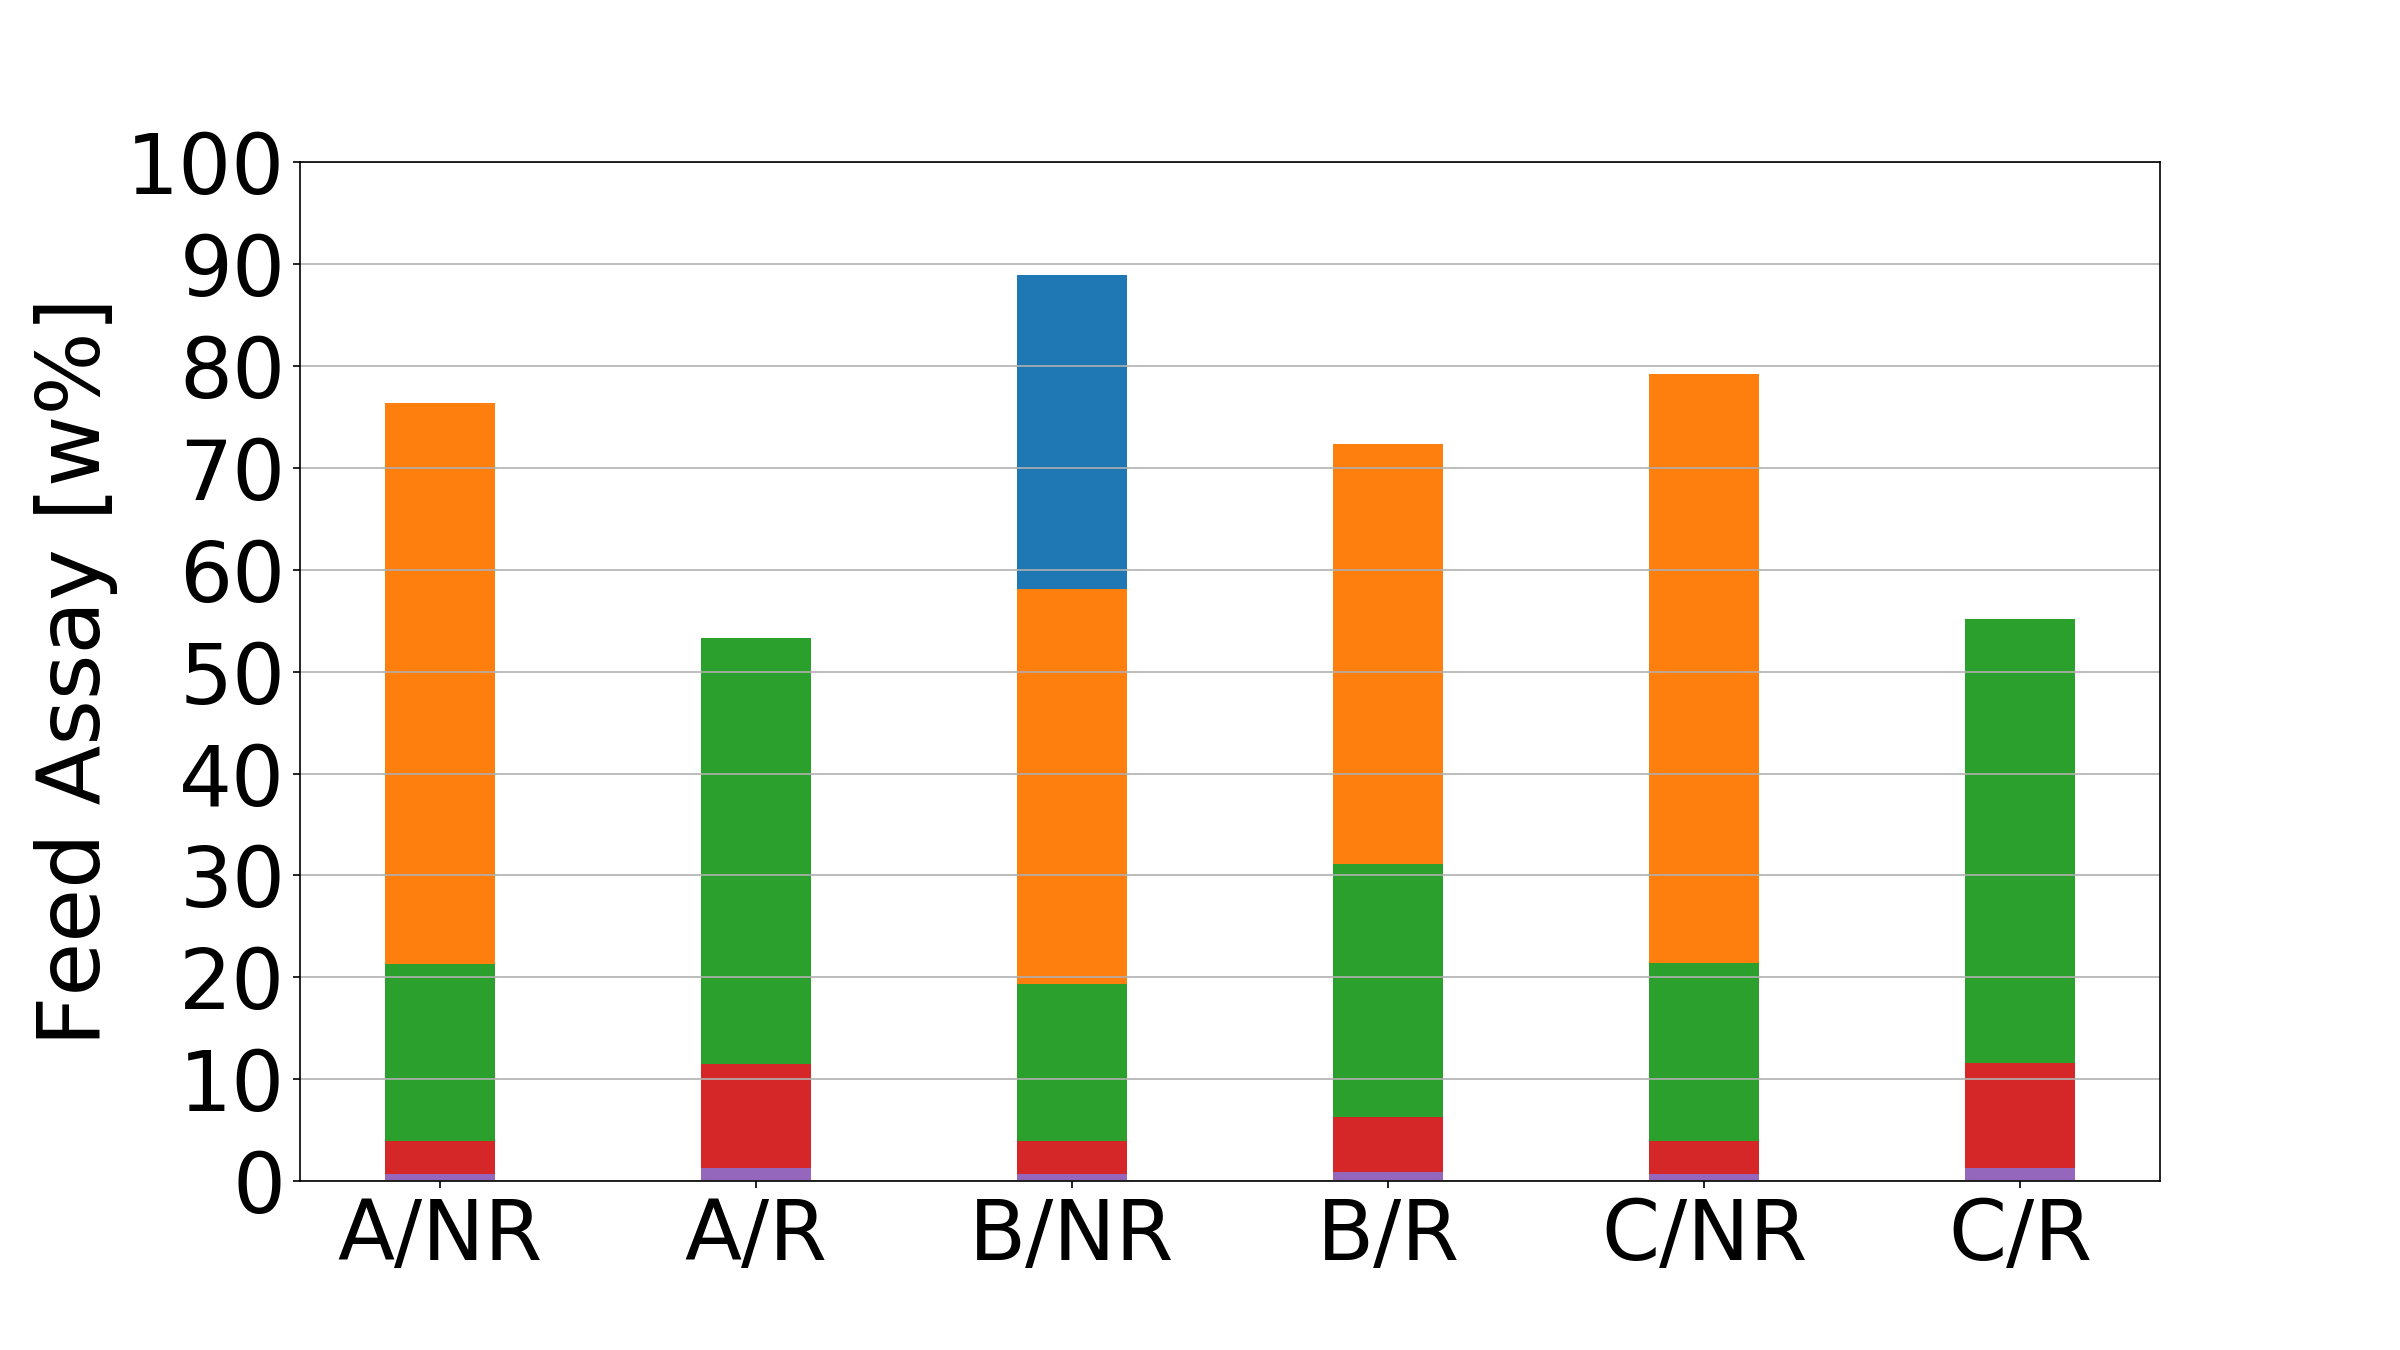
\includegraphics[width=\linewidth]{feed_assays}
        \caption{Feed Assays}
        \label{sfig:feed_assay}
    \end{subfigure}%
    \begin{subfigure}[t]{0.45\textwidth}
        \centering
        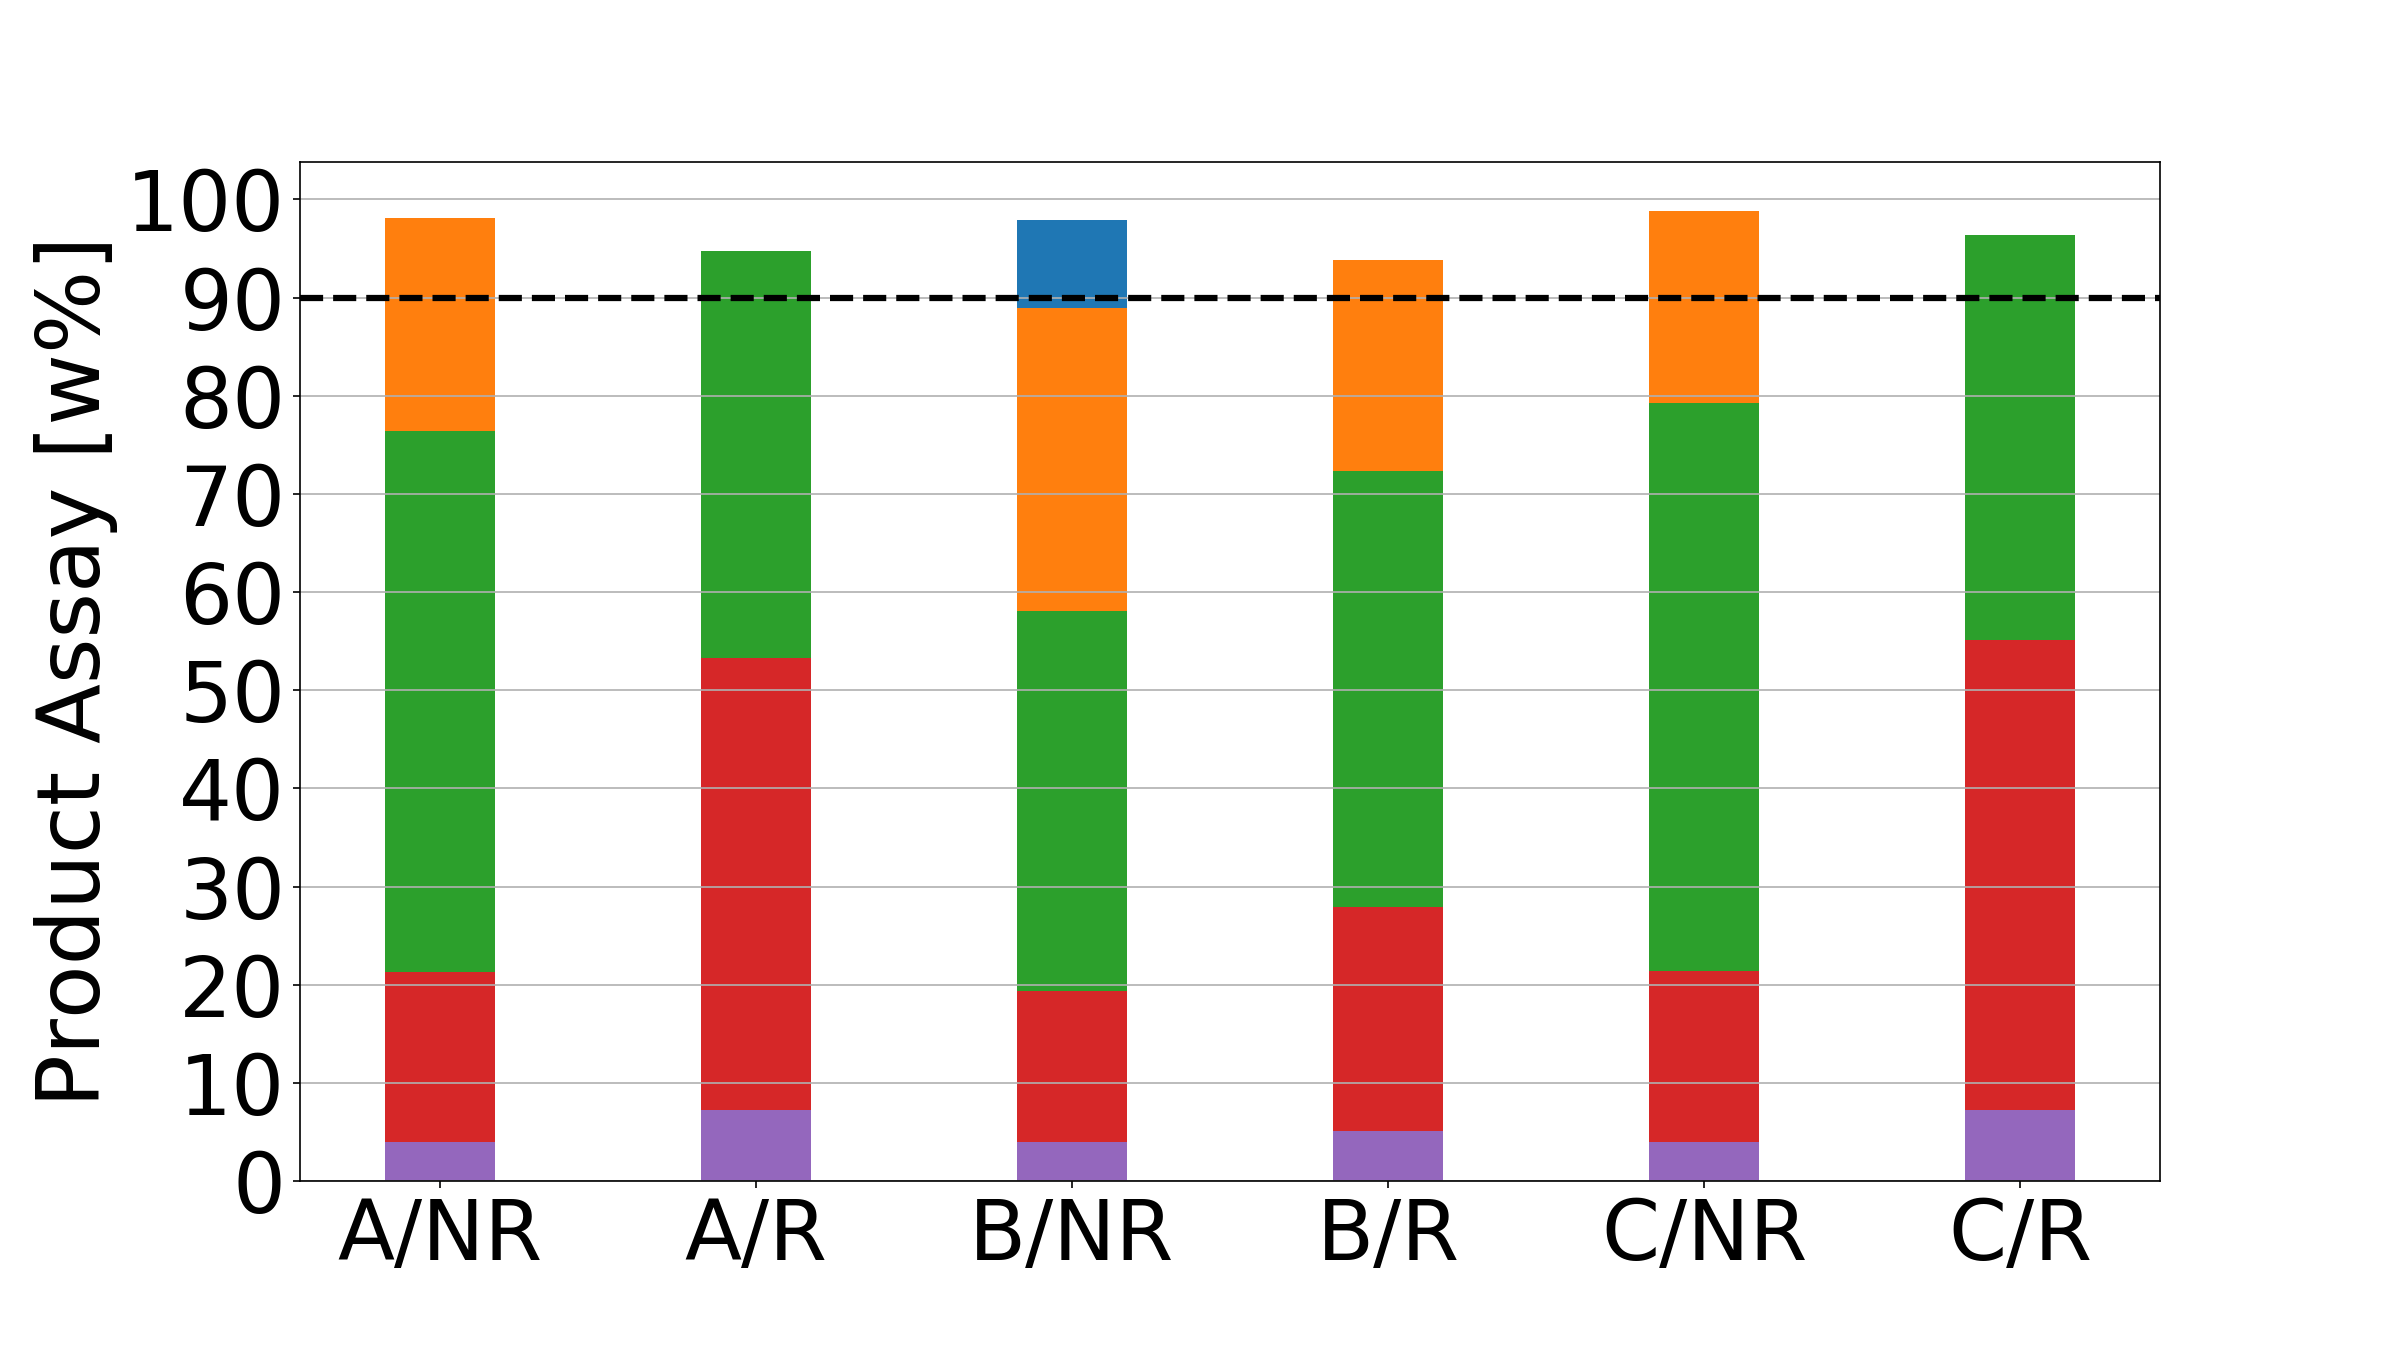
\includegraphics[width=\linewidth]{product_assays}
        \caption{Product Assays}
        \label{sfig:product_assay}
    \end{subfigure}
    \begin{subfigure}[t]{0.45\textwidth}
        \centering
        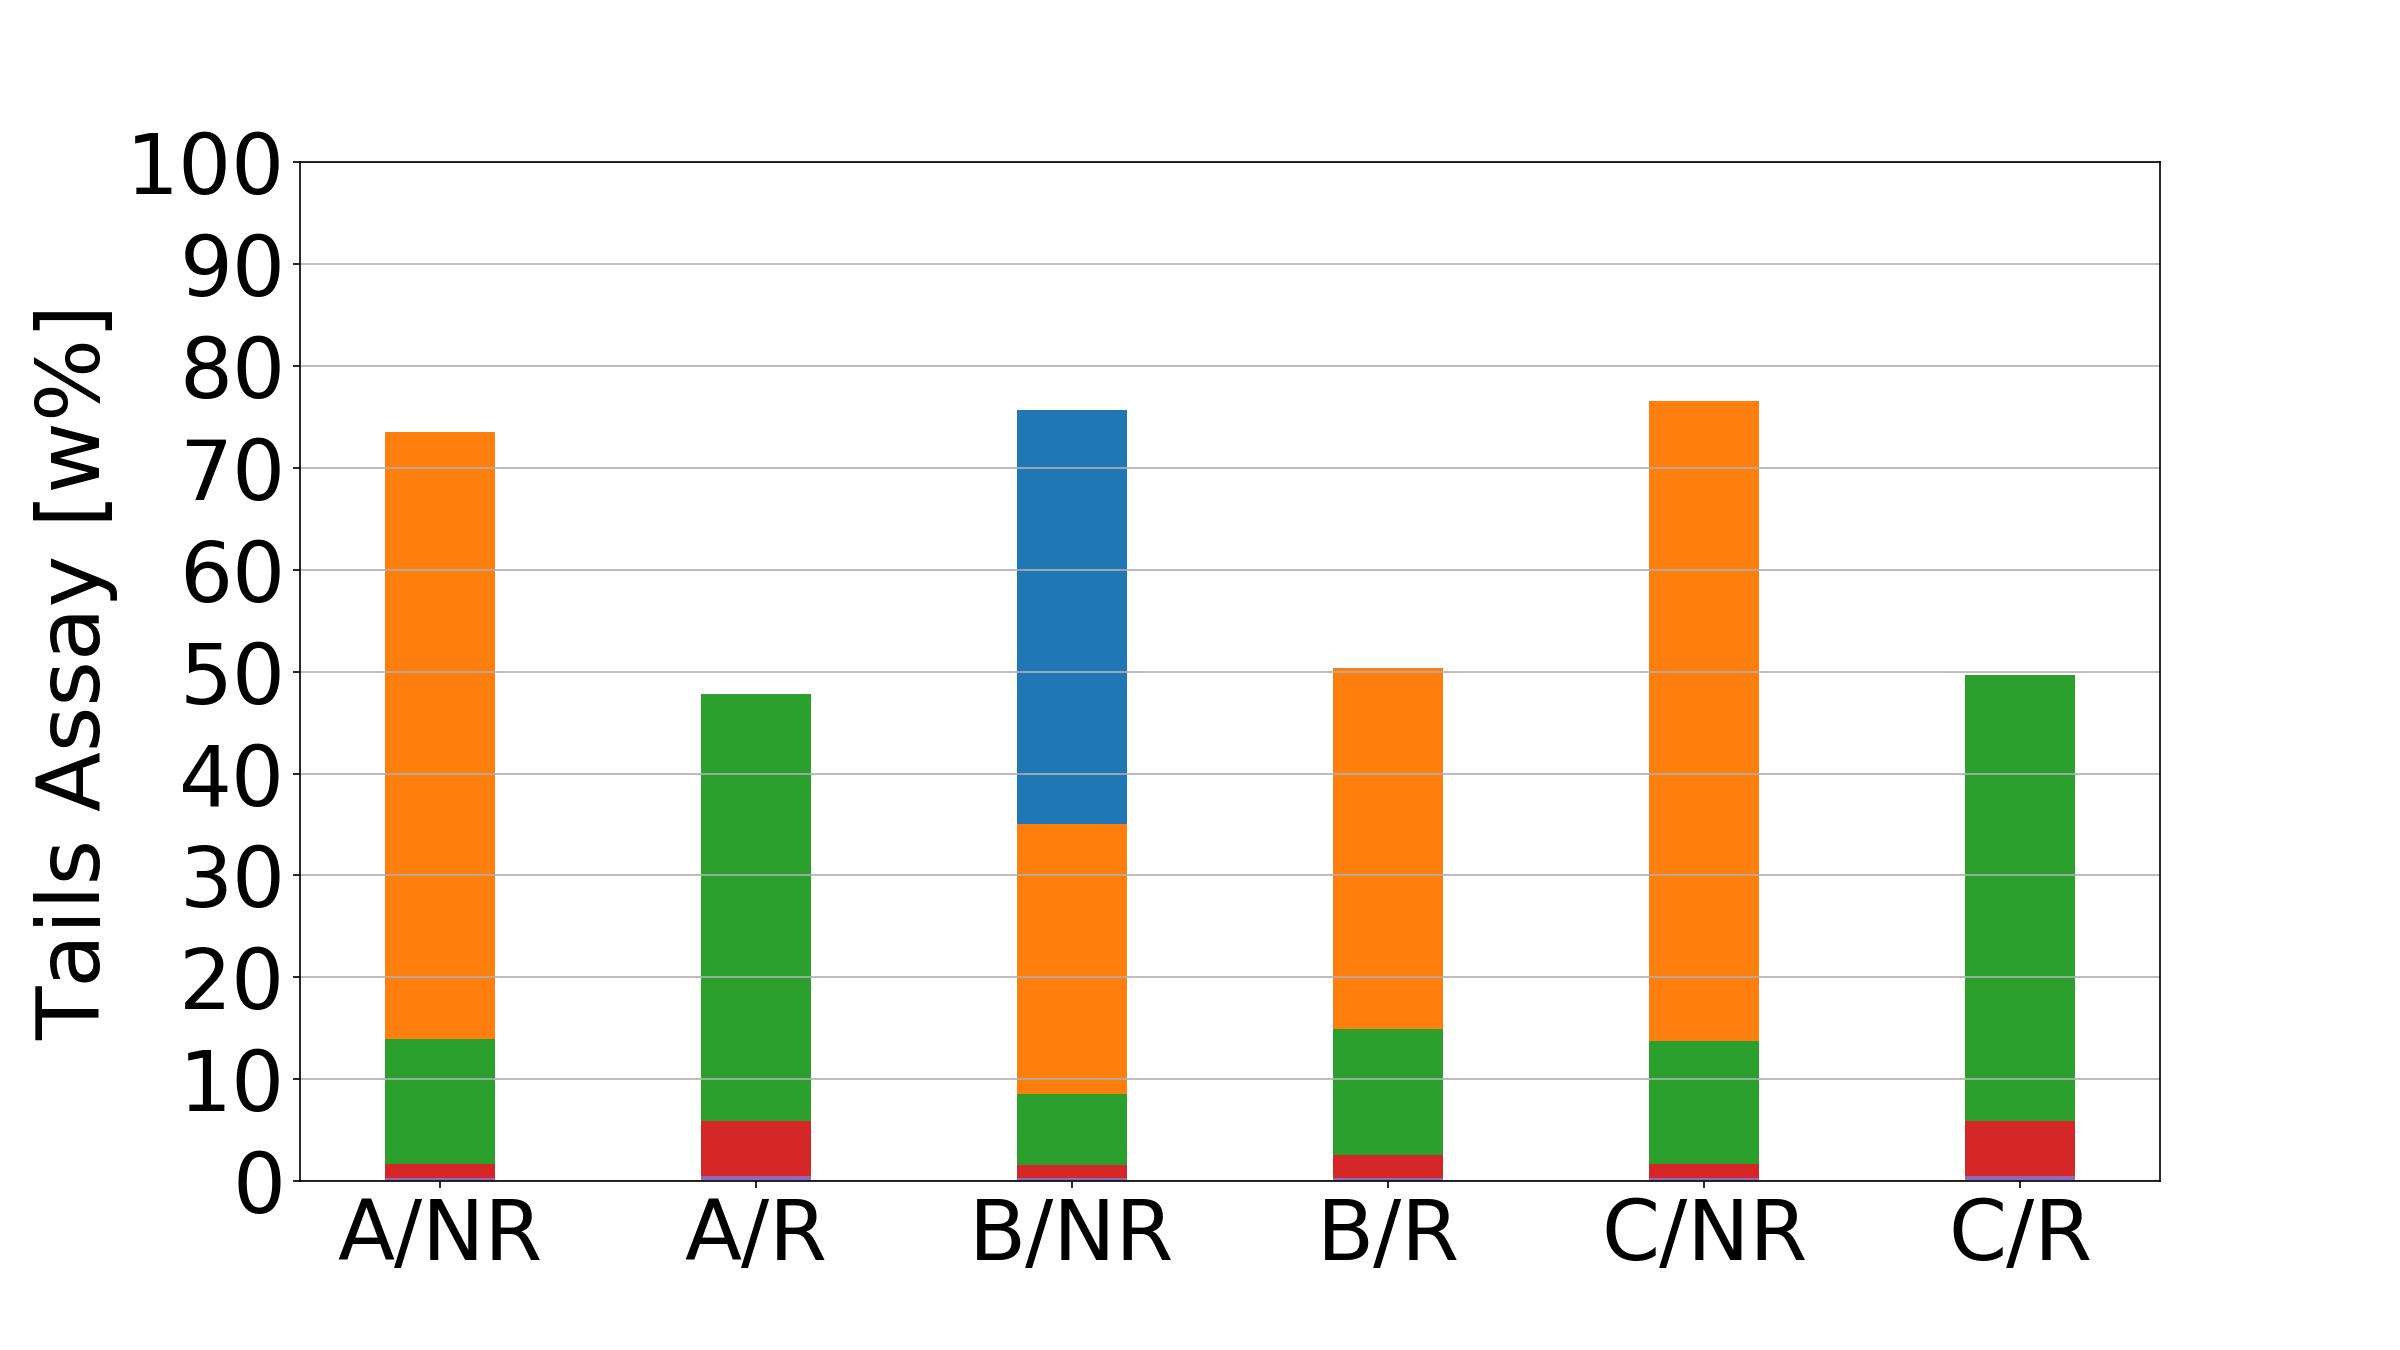
\includegraphics[width=\linewidth]{tails_assays}
        \caption{Tails Assays}
        \label{sfig:tails_assay}
    \end{subfigure}
    \caption{Feed (\subref{sfig:feed_assay}), product
        (\subref{sfig:product_assay}) and tails assays (\subref{sfig:tails_assay})
        in $w\%$ of $^{235}$U, per cascade level from 0 to 3 (red, green, orange,
        blue), per model (A/B/C) and without/with tails recycling (NR/R). The
        black dashed line represents the $90 w\%$ enrichment threshold.}
    \label{fig:assays}
\end{figure}



\subsection{Tails recycling}

As shown in Figures \ref{fig:assays}, recycling the tails increases the overall product assay at
all the different levels. As the tails assay of a level $n+1$ is always higher than
the product assay of the level $n-1$, recycling the tails of level $n+1$ will
consequently increase the feed assay of level $n$ (see Table \ref{tab:level}).
Moreover, with an increased feed assay, tails and product assays increase as
well, increasing de facto the feed assays of respectively cascade levels $n-1$
and $n+1$, etc.  This effect reduces the number of cascade levels required to reach
\gls{HEU} in case A and C.



\subsection{\gls{HEU} Production Rate}

As shown in Figure \ref{fig:HEU_rate}, recycling increases the final \gls{HEU}
production rate, from $2$ to almost $20$ kg/y when using models A and C, and from
$17$ to $38$ kg/y with the model B. For the reference calculation where all the
available cascades are used within a single large cascade design for direct
\gls{HEU} production, the \gls{HEU} production rate is slightly over $50$ kg/y.


As models A and C, rely on maintaining the cut values at each stages of the
cascade and share the same number of levels, have the exact same cascade
repartition across the different levels and the same \gls{HEU} production rate.

\begin{figure}[h!] % replace 't' with 'b' to force it to be on the bottom
    \centering
    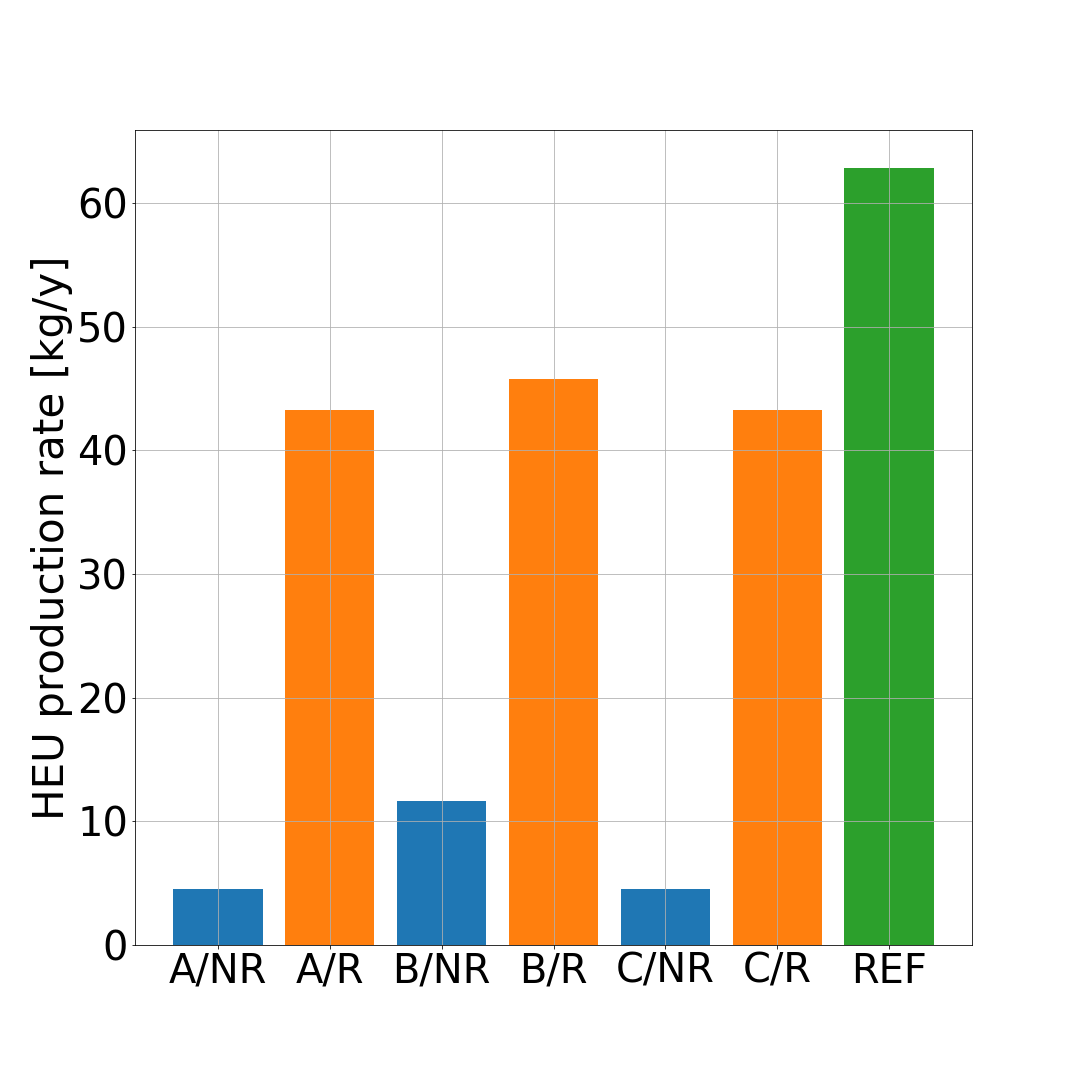
\includegraphics[scale=0.25]{HEU_prod_rate}
    \caption{Production rate at equilibrium for the different model
        configurations, the case without tails recycling (blue), with tails
        recycling (orange), and the reference one (green). A-B-C represent
        the model used, and NR-R the case without tails recycling and the case
        with tails recycling, respectively.}
    \label{fig:HEU_rate}
\end{figure}
